% ============================================================================
% M4 section -- PNAS template (pnas-new.cls, Overleaf)
% Paste into the main .tex where the section belongs.
% Requires: graphicx and amsmath (already loaded by pnas-new.cls).
% Upload m4_cs_event_rent_en.png to the Overleaf project (same folder as main.tex,
% or adjust the path in \includegraphics) and add m4_refs.bib entries to the
% project bibliography.
% Numbers: output/tables/m4_cs_results.csv, m4_ci_inversion.csv, m4_power.csv,
% m4_robustness.csv, m4_timing_robustness.csv, m4_sdid_cs_compare.csv,
% m4_sdid_results.csv, m4_event_study.csv (modules 19--19h).
% ============================================================================

\section*{The M4 Metro Line and Local Rents}

In the five OMI zones that gained new access, over the first three to seven semesters after opening, we find no robust evidence that Milan's M4 metro line raised rent quotations relative to comparable zones. This section asks whether the M4, opened in three stages between November 2022 and October 2024, changed residential rents in the zones it served for the first time.

The standard prediction comes from the capitalisation of accessibility: better transit access lowers commuting costs, and households bid up housing close to new stations \cite{alonso1964,gibbons2005}. Empirical studies of new rail lines generally find positive but modest and very local effects, which decay quickly with distance from the station \cite{billings2011}. In the Italian context, Daniele and Romito \cite{daniele2022} study Metro C in Rome with the same OMI data used here. If rents rise near new stations, the line would contribute to the affordability pressures documented in the previous sections.

Milan offers a staggered natural experiment: three sections of the same line opened at different dates. We exploit this timing with the heterogeneity-robust difference-in-differences estimator of Callaway and Sant'Anna \cite{callaway2021} and an event-study design. Because only five zones are treated, we base inference on permutation and report the minimum detectable effect. Relative to matched controls, rents in newly served zones grew 4.6\% less after opening (95\% CI $-9.7\%$ to $+2.2\%$; permutation $p=0.13$). The event study shows that the relative decline of the served zones began years before opening, so the negative estimate should not be read as a causal fall in rents. Results are similar with all never-exposed zones as controls, with alternative catchments and exposure thresholds, without any single treated zone, and with a synthetic difference-in-differences estimator ($-3.8\%$).

\subsection*{Data}

Rents come from the semi-annual quotations of the Osservatorio del Mercato Immobiliare (OMI) of the Agenzia delle Entrate. For each OMI zone and semester, OMI publishes a minimum and a maximum value for residential units (\textit{abitazioni civili}) in normal condition; we use the midpoint of the range of the monthly rent, in euros per square metre of gross floor area. The panel runs from 2014S2 to 2026S1: earlier semesters use a different zoning map, and 2014S1 is a transition semester in which part of the city still carries the old zone codes. We keep the zones with a rent quotation in every semester, a balanced panel of 37 zones. The 2026S1 semester, not yet in the municipal open-data release, is taken directly from the Agenzia delle Entrate. Values are nominal; deflating by a price index common to all zones would leave every estimate below unchanged, because the common term cancels in the double difference (we verified this numerically).

To select comparable control zones we use 2014 municipal registry data on the shares of foreign residents, of residents aged 65 and over, and of single-person households, by neighbourhood (\textit{Nuclei di Identit\`a Locale}, NIL), mapped to OMI zones by area overlap. Station coordinates and line membership come from the municipal open-data portal (dataset ds535); each M4 station is assigned to the section that served it at opening.

\subsection*{Treatment Definition and Timing}

An area is treated when at least 20\% of its surface gains new metro access within 500 metres of an M4 station. We overlay a regular grid of points on the city. A point is \textit{newly served} if it lies within 500~m of an M4 station and more than 500~m from any station of the other lines (M1, M2, M3, M5). An area's exposure to a section is the share of its grid points newly served by that section's stations. An area is treated if its exposure reaches 20\%, and \textit{never exposed} if no point lies within 500~m of any M4 station; partially exposed areas, and areas near the M4 already served by other lines, are excluded. The 500~m radius matches the walking catchment of an urban station, is close to the median distance between consecutive M4 stations (469~m), and halves the minimum detectable effect relative to 800~m.

The first treated period is the first semester during which the section was open for all or almost all of the period (Table~\ref{tab:m4timing}). Section 2 serves no zone for the first time, because Tricolore and San Babila are within 500~m of the M1 and M3 lines. Five OMI zones are therefore treated: one from 2023S1, with seven post-opening semesters, and four from 2025S1, with three.

\begin{table*}[tbhp]
\centering
\caption{Opening dates and treated OMI zones (500~m catchment, 20\% exposure threshold)}
\label{tab:m4timing}
\resizebox{\textwidth}{!}{%
\begin{tabular}{llcccl}
\hline
Section & Opening & Opening semester & First treated & Post-opening semesters & Treated zones \\
 & & (share of days open) & semester & to 2026S1 & \\
\hline
1 Linate--Dateo & 26 Nov 2022 & 2022S2 (20\%) & 2023S1 & 7 & 1 (D12) \\
2 Dateo--San Babila & 4 Jul 2023 & 2023S2 (98\%) & 2023S2 & 6 & 0 \\
3 San Babila--San Cristoforo & 12 Oct 2024 & 2024S2 (44\%) & 2025S1 & 3 & 4 (B13, B20, B21, D24) \\
\hline
\end{tabular}}
\addtabletext{Source: authors' elaboration on OMI and municipal open data.}
\end{table*}

\subsection*{Empirical Strategy}

We estimate group-time average treatment effects with the estimator of Callaway and Sant'Anna \cite{callaway2021}, which compares each opening group only with units that are not yet, or never, treated.

\paragraph{Target parameter and identifying assumptions.} The estimand is the average effect of gaining new M4 access on the log OMI midpoint rent of the five treated zones, over the semesters observed after their opening and weighted as described below, relative to the counterfactual path given by the controls. Its identification requires (\textit{i}) parallel trends: absent the line, treated zones and their controls would have followed the same rent path from the reference semester onwards; (\textit{ii}) no anticipation between the reference semester and opening; and (\textit{iii}) no spillovers of the line onto the control zones. Three consequences follow. The estimate is a relative effect, so any effect of the line common to all zones of the city is differenced out; it concerns OMI quotations, which are appraisal-based ranges rather than transaction rents; and it says nothing about effects beyond the observed three to seven semesters.

\paragraph{Why not two-way fixed effects.} With staggered adoption, a two-way fixed-effects regression of the outcome on a treatment dummy uses already-treated units as controls for later-treated ones, which can bias the estimate in either direction when effects vary over time \cite{goodmanbacon2021,dechaisemartin2020}. We report the two-way estimate, with zone fixed effects and one fixed effect for each calendar semester, only for comparison.

\paragraph{Group-time effects and aggregation.} Let $g$ be the first treated period of a group and $b=g-1$ a common reference period. For log rent $Y$,
\begin{equation}
\mathrm{ATT}(g,t)=\left[\bar Y_{g,t}-\bar Y_{g,b}\right]-\left[\bar Y_{C(g,t),t}-\bar Y_{C(g,t),b}\right],
\label{eq:attgt}
\end{equation}
where the control set $C(g,t)$ contains the sample units that are never exposed or that open after $\max(t,b)$, and means are unweighted across units. The headline estimate averages the post-opening effects, weighting each group by its number of treated units $n_g$:
\begin{equation}
\mathrm{ATT}=\frac{\sum_g\sum_{t\ge g} n_g\,\mathrm{ATT}(g,t)}{\sum_g\sum_{t\ge g} n_g}.
\label{eq:attagg}
\end{equation}
The first section (one zone $\times$ 7 semesters) thus receives weight 7/19 and the third section (four zones $\times$ 3 semesters) 12/19. Aggregating by time relative to opening, $e=t-g$, gives the event study
\begin{equation}
\mathrm{ES}(e)=\frac{\sum_g n_g\,\mathrm{ATT}(g,g+e)}{\sum_g n_g},
\label{eq:es}
\end{equation}
where the sums run over the groups observed at $e$ and $\mathrm{ES}(-1)=0$ by construction. Pre-opening coefficients test for differential trends; their average over $e=-8,\dots,-2$ is reported as a placebo.

\paragraph{Three specifications.} The estimator, outcome and sample period are the same in all three; only the control group changes.
\begin{enumerate}
\item \textit{Matched + not-yet-treated (main).} For each treated zone we take the three never-exposed zones most similar before the metro, by Euclidean distance on standardised covariates: the 2014--2016 levels of log rents and log prices, the 2014--2019 growth of log rents, and the 2014 shares of foreign residents, residents aged 65 and over, and single-person households. This yields six matched controls. Zones of later sections are added as not-yet-treated controls until they open.
\item \textit{All never-exposed + not-yet-treated.} As (1), with all 20 never-exposed zones as controls; it tests whether the result depends on the matching.
\item \textit{Not-yet-treated only.} Only zones of sections that open later serve as controls. They were selected by the same planning process and are natural candidates for the route. Once the last section opens no control is left, so this specification compares the single section-1 zone with the four section-3 zones up to 2024S2.
\end{enumerate}

\subsection*{Inference and Statistical Power}

With five treated zones, cluster-robust standard errors are unreliable \cite{conley2011,mackinnon2018}, so we base inference on randomisation. We test the sharp null that the M4 had no effect on any zone in any semester. Under this null the label ``treated'' carries no information, and assigning the opening dates to other zones would produce estimates of the same kind. In the main sample of 11 zones we randomly reassign the labels (one zone opening in 2023S1, four in 2025S1, six controls), keeping the number of zones per group fixed, and recompute the full estimator for each of 999 draws; there are 2,310 distinct assignments. The two-sided $p$-value is $p=(1+\#\{|\mathrm{ATT}_p|\ge|\mathrm{ATT}|\})/(1+B)$, with $B$ the number of draws; the same procedure gives the $p$-value of the pre-opening placebo.

This $p$-value has exact finite-sample level only if, under the null, the observed assignment of opening dates is one equally likely draw among the relabellings of the 11 zones; with randomly drawn permutations, $p=(1+b)/(1+B)$ keeps this property. The opening dates were set by the route of the line, not randomised, and the treated zones are central, so exchangeability is a maintained assumption rather than a feature of the design. The test also conditions on the selected sample: the matched controls were chosen with knowledge of the treated zones, and matching is not repeated within permutations.

For the three specifications in Table~\ref{tab:m4main} we obtain 95\% confidence intervals by inverting the permutation test under a constant additive effect $\tau$ \cite{imbens2015}. A value $\delta$ belongs to the interval if the permutation test of no effect, applied to $Y-\delta D$ with $D=1$ for treated zones after their own opening, does not reject at 5\%; the endpoints are found by bisection, using the same 999 permutations for every $\delta$. For robustness checks and event-study coefficients we use a faster approximation, the estimate $\pm c$, where $c$ is the 95th percentile of the permuted $|$estimates$|$; it treats the permutation distribution under $\tau=0$ as if it did not change with $\tau$. For the main specification it gives $[-10.4\%,+1.7\%]$ against the exact $[-9.7\%,+2.2\%]$.

For the event study we report pointwise intervals $\mathrm{ES}(e)\pm c_e$ and a simultaneous band $\mathrm{ES}(e)\pm\hat c\,\mathrm{sd}_e$, where $\mathrm{sd}_e$ is the standard deviation of the permuted coefficients at $e$ and $\hat c$ is the 95th percentile, across permutations, of $\max_e|\mathrm{ES}_p(e)|/\mathrm{sd}_e$ over $e=-12,\dots,6$, excluding the reference $e=-1$ ($\hat c=2.40$). The band follows the sup-$t$ logic of Montiel Olea and Plagborg-M{\o}ller \cite{montielolea2019}, applied to the permutation distribution rather than to a bootstrap; its joint coverage of all pre- and post-opening coefficients holds under the same constant-effect approximation.

Under the same approximation, from the permutation distribution $e$ we compute the minimum detectable effect (MDE) with 80\% power, the smallest $\delta$ such that $P(|\delta+e|\ge c)\ge0.8$. In the main specification $c=0.062$ log points and the MDE is 9.4\% (9.2\% with all never-exposed controls). A non-significant estimate therefore means that an effect of about $\pm9\%$ would have been detected in eight cases out of ten; smaller effects, of the size found in part of the literature, cannot be ruled out. The MDE has a Monte Carlo error of about 0.3 percentage points and is not monotone in the length of the post-period (8.7\% to 2025S2, 9.4\% to 2026S1): adding a semester does not mechanically increase precision when quotations move in persistent steps.

\subsection*{Results}

None of the three specifications shows an increase in rents after the M4 opened (Table~\ref{tab:m4main}). The two specifications that use never-exposed controls give negative estimates of 4--5\%, with confidence intervals that include zero.

\begin{table*}[tbhp]
\centering
\caption{Effect of the M4 opening on log rents: Callaway--Sant'Anna estimates}
\label{tab:m4main}
\resizebox{\textwidth}{!}{%
\begin{tabular}{llcccccc}
\hline
 & Controls & ATT & 95\% CI & Permutation & Pre-opening & Treated / never- & Period \\
 & & & & $p$ & placebo ($p$) & exposed controls & \\
\hline
(1) Main & Matched + not-yet-treated & $-4.6\%$ & $[-9.7\%, +2.2\%]$ & 0.133 & $+0.028$ (0.52) & 5 / 6 & 2014S2--2026S1 \\
(2) & All never-exposed + not-yet-treated & $-4.0\%$ & $[-9.6\%, +2.4\%]$ & 0.243 & $+0.052$ (0.20) & 5 / 20 & 2014S2--2026S1 \\
(3) & Not-yet-treated only & $+3.2\%$ & $[-4.6\%, +11.7\%]^{a}$ & 0.625 & $-0.045$ (0.62) & 5 / 0 & 2014S2--2024S2 \\
\hline
\end{tabular}}
\addtabletext{Outcome: log of the OMI midpoint rent; OMI zones, semesters. Percentages are $100\times(\exp(\mathrm{ATT})-1)$. Permutation $p$-values use 999 random relabellings of the opening groups. 95\% intervals invert the permutation test under a constant additive effect; $^{a}$approximate interval (estimate $\pm c$). The placebo is the average pre-opening coefficient over $e=-8,\dots,-2$, in log points. In (3), the four section-3 zones are controls for the section-1 zone until they open, so the window ends in 2024S2.}
\end{table*}

In the main specification, rents in newly served zones grew 4.6\% less than in matched controls after opening ($p=0.13$). Under the constant-effect assumption, effects outside $[-9.7\%,+2.2\%]$ are rejected at the 5\% level: rent increases larger than about 2\% are inconsistent with the data, while decreases of up to about 10\% cannot be ruled out. With all never-exposed controls the estimate is very similar ($-4.0\%$), so the result does not depend on the matching. The not-yet-treated-only estimate is positive but very imprecise ($+3.2\%$, CI $-4.6\%$ to $+11.7\%$); it rests on one treated zone compared with four zones that open later, over four post-opening semesters, and we treat it as uninformative rather than as contradicting (1) and (2). A two-way fixed-effects regression with zone and semester fixed effects gives $-12.2\%$. The gap with Callaway--Sant'Anna comes mainly from the reference period: the two-way model compares post-opening rents with the average of all pre-opening semesters, during which the served zones were declining relative to the controls.

\begin{figure*}[tbhp]
\centering
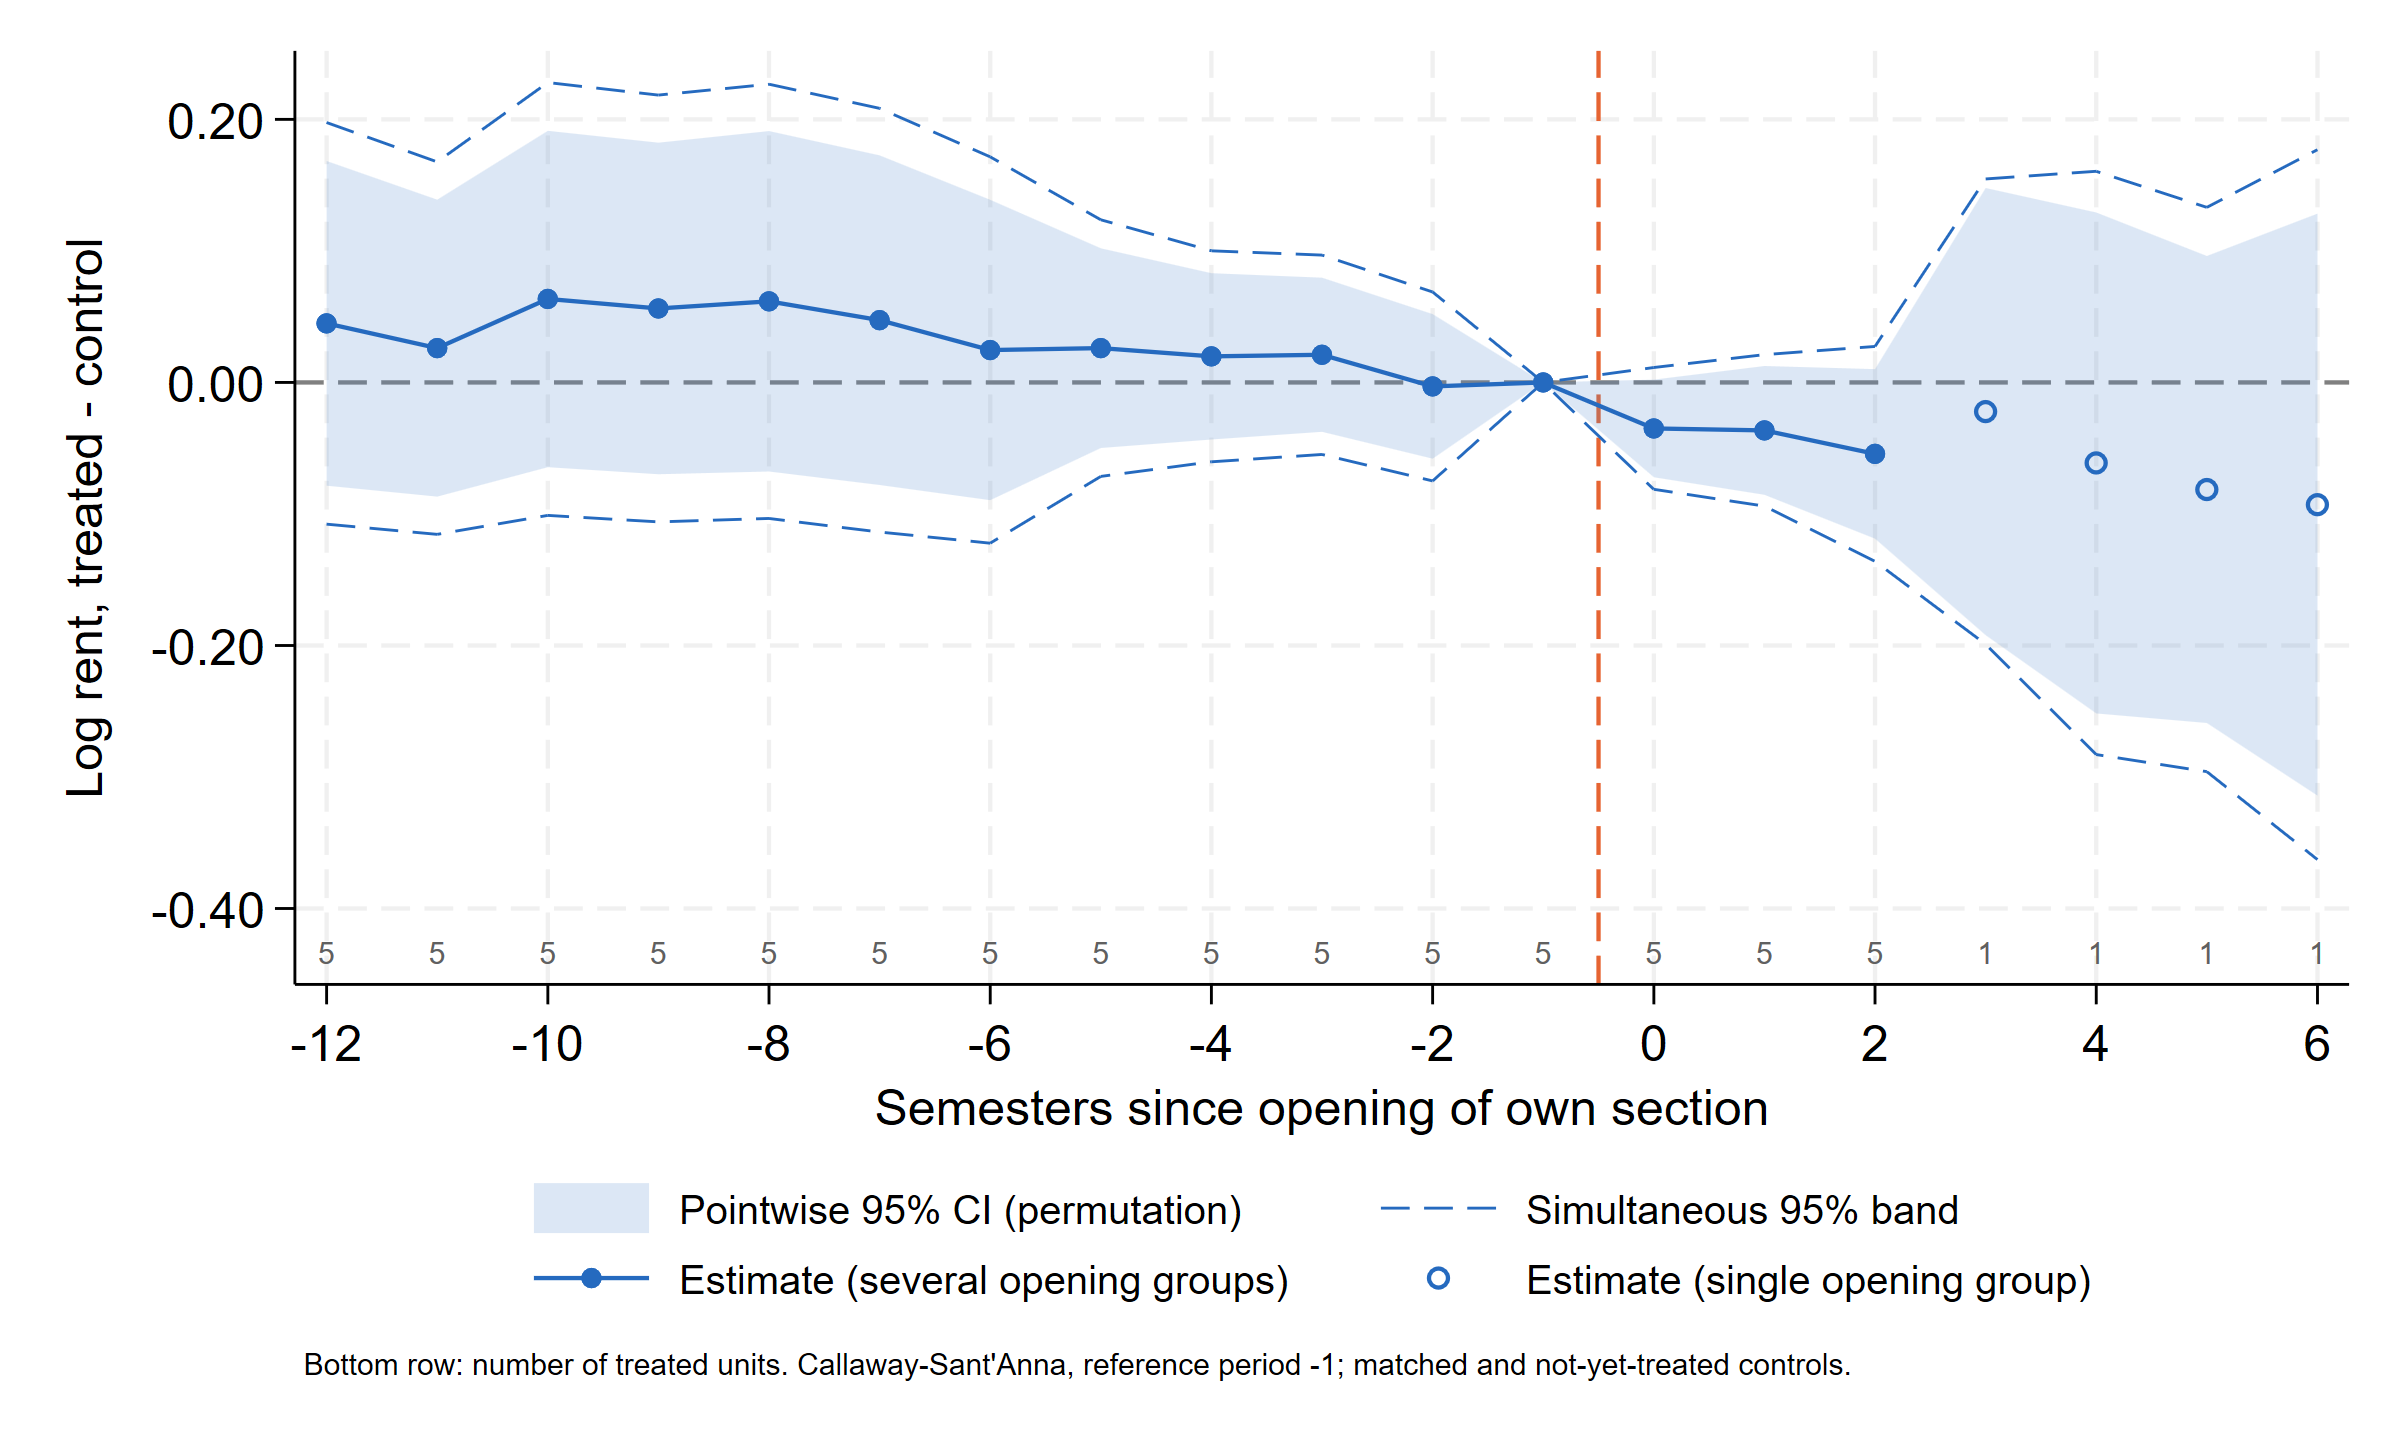
\includegraphics[width=0.8\textwidth]{m4_cs_event_rent_en.png}
\caption{Event study: log rent, newly served zones vs.\ matched and not-yet-treated controls. Callaway--Sant'Anna coefficients by semester relative to opening (reference $e=-1$). Shaded area: approximate pointwise 95\% intervals (estimate $\pm c_e$); dashed lines: approximate 95\% simultaneous sup-$t$ band over $e=-12,\dots,6$, both from 999 permutations of the opening groups. Bottom row: number of treated zones in each coefficient; hollow markers rest on a single opening group.}
\label{fig:m4event}
\end{figure*}

Figure~\ref{fig:m4event} shows the event study. Before opening, rents in M4 zones were 4 to 6 log points above matched controls up to $e=-7$ and converged steadily to zero by $e=-1$. No pre-opening coefficient is individually significant, and the simultaneous band contains zero for all of them; the point estimates nonetheless trace a gradual relative decline that started years before the line opened, and the pre-test has little power with five treated zones. After opening, the first three coefficients are $-0.035$ (95\% CI $-0.072$ to $+0.002$), $-0.036$ and $-0.054$, all with intervals that include zero. From $e=+3$ to $+6$ the coefficients rest on a single zone (D12, section 1), so the further fall to $-0.09$ reflects the change in composition, not a growing effect. Taken together, the post-opening decline is consistent with the continuation of the pre-existing trend. The design cannot separate a possible effect of the line from that trend, so the negative coefficients are not evidence of a causal fall in rents.

We also examined OMI sale prices and resident out-migration at the neighbourhood level with the same design. Neither shows a robust effect: prices $-3.1\%$ ($p=0.27$); out-migration $-2.4$ per 1,000 residents ($p=0.07$), which falls to $-1.0$ ($p=0.51$) with an earlier reference year. We do not report them further.

\subsection*{Robustness}

The rent estimate stays between $-1\%$ and $-6\%$ across alternative treatment definitions, samples, reference periods and estimators (Table~\ref{tab:m4robust}).

\begin{table}[tbhp]
\centering
\caption{Robustness checks, log rent}
\label{tab:m4robust}
\begin{tabular}{lccc}
\hline
Check & Estimate & $p$ & Treated \\
\hline
Main specification (1) & $-4.6\%$ & 0.13 & 5 \\
Catchment 800 m & $-5.2\%$ & 0.42 & 3 \\
Catchment 1,000 m & $-1.3\%$ & 0.80 & 4 \\
Exposure threshold 10\% & $-4.6\%$ & 0.036 & 10 \\
Exposure threshold 30\% & $-4.2\%$ & 0.32 & 2 \\
Leave one treated zone out & $-3.6$ to $-5.6\%$ & 0.05--0.23 & 4 \\
Reference period $g-2$ & $-4.4\%$ & 0.40 & 5 \\
Treatment from opening semester & $-3.5\%$ & 0.45 & 5 \\
Synthetic DiD & $-3.8\%$ & 0.27 & 5 \\
\hline
\end{tabular}
\addtabletext{Callaway--Sant'Anna with matched and not-yet-treated controls and permutation $p$-values, unless stated. Catchment and threshold variants use 499 permutations. The synthetic DiD uses all never-exposed zones; its $p$-value comes from placebo standard errors and a normal approximation, not from the permutation test.}
\end{table}

\paragraph{Treatment definition and influential units.} The estimate is similar with an 800~m catchment or a 10\% or 30\% exposure threshold, and smaller with a 1,000~m catchment. With the 10\% threshold the number of treated zones doubles and the estimate becomes significant ($-4.6\%$, $p=0.036$), with the same sign and size as the main estimate. Dropping one treated zone at a time keeps the estimate between $-3.6\%$ and $-5.6\%$.

\paragraph{Classification of opening periods.} The reference semester is partly treated for two sections: 2022S2 was served for 20\% of its days (section 1) and 2024S2 for 44\% (section 3). Using $g-2$ as reference, so that the partially treated period enters neither the base nor the effects, or dating treatment from the opening semester itself, leaves the estimate unchanged ($-4.4\%$ and $-3.5\%$).

\paragraph{Synthetic difference-in-differences.} The estimator of Arkhangelsky et al.\ \cite{arkhangelsky2021} reweights controls and pre-opening periods so that the control group tracks the treated zones before opening. On the same balanced sample and horizon (5 treated, 20 never-exposed zones), it gives an estimate close to Callaway--Sant'Anna and insignificant (Table~\ref{tab:m4sdid}). The pre-trend is the mean of $[(\text{treated}-\text{control})_t-(\text{treated}-\text{control})_{g-1}]$ over $e=-8,\dots,-2$, measured in the same way for all methods. Unit weights spread over about 11 effective controls, with a maximum weight of 0.17; time weights concentrate on the semester before opening (66\% for section 1, 97\% for section 3).

\begin{table}[tbhp]
\centering
\caption{Same sample and horizon: Callaway--Sant'Anna, difference-in-differences and synthetic DiD}
\label{tab:m4sdid}
\resizebox{\columnwidth}{!}{%
\begin{tabular}{lcccc}
\hline
Method & Estimate & 95\% CI & $p$ & Pre-trend \\
\hline
C\&S, never-exposed controls & $-4.1\%$ & $[-10.4\%, +2.7\%]$ & 0.23 & $+0.054$ \\
Difference-in-differences & $-12.5\%$ & $[-21.6\%, -2.4\%]$ & 0.017 & $+0.054$ \\
Synthetic DiD & $-3.8\%$ & $[-10.2\%, +3.0\%]$ & 0.27 & $+0.015$ \\
\hline
\end{tabular}}
\addtabletext{5 treated and 20 never-exposed zones, 2014S2--2026S1. C\&S: permutation $p$ and approximate interval (estimate $\pm c$); difference-in-differences and synthetic DiD: placebo standard errors (500 replications) and normal approximation.}
\end{table}

\subsection*{Limitations and Interpretation}

Under the maintained assumptions, the estimates are inconsistent with relative rent increases larger than about 2\%, but they cannot distinguish a zero effect from a moderate decrease. Six features of the setting limit what they can show. First, five OMI zones carry the estimates; the permutation $p$-value has exact level only if opening dates are exchangeable across the sample zones, which the route of the line does not guarantee, intervals other than those in Table~\ref{tab:m4main} are approximate, and power reaches 80\% only for effects of about $\pm9\%$. Second, the post-period is short: seven semesters for section 1 and three for section 3. Third, newly served zones are mostly central, while clean controls, especially those more than 2~km from the line, are peripheral; any divergence between centre and periphery over the same years is confounded with the effect of the line, and the positive pre-opening placebo points in this direction. Fourth, the semester before the first treated one was already partly served for two sections, although excluding it does not change the estimate. Fifth, the line was announced and construction began before 2014, so any capitalisation at announcement predates our panel. Sixth, an OMI zone is much larger than a station's catchment, which dilutes a local effect; station-level listing data could sharpen the estimates but are outside the scope of this paper.

The appropriate reading is therefore that, in the sample and horizon observed, we find no robust evidence that the M4 raised OMI rents. It is not that the M4 had no effect, nor that it lowered rents.

\subsection*{Conclusion}

In the five newly served OMI zones and over the first three to seven semesters after opening, we find no robust evidence of an increase in OMI rent quotations, relative to comparable zones, attributable to the opening of the M4. The central Callaway--Sant'Anna and synthetic difference-in-differences estimates are negative ($-4.6\%$ and $-3.8\%$), but uncertainty and the limits of the comparison prevent reading them either as proof of a zero effect or as a causal reduction in rents: the relative decline of the served zones began before the line opened. For the affordability question of this paper, the 2022--2024 rise in rents documented earlier does not appear concentrated in the zones newly served by the M4. Because the design identifies a relative effect, it cannot speak to effects of the line common to the whole city. Longer post-periods and finer spatial data will allow a sharper test.
